\documentclass[11pt,a4paper]{article}
\usepackage[T1]{fontenc}
\usepackage[utf8]{inputenc}
\usepackage{lmodern}
\usepackage[margin=25mm]{geometry}
\usepackage{graphicx,booktabs,amsmath,float}
\usepackage[hidelinks]{hyperref}
\graphicspath{{fig/}{../results/}{../cad/}}

\title{Technical assignment: pick and place of U-profiles with two xArm6\\ \large (drawing AMZ-SA-26-001)}
\author{Ilya Mashkov}
\date{November 2026}

\begin{document}
\maketitle

\section{Task and short summary}
Two UFACTORY xArm6 robots have to pick four U-profiles and place them into the hash assembly from the drawing. The second question is how the tolerances of 0.05~mm can be reached, if the robots themselves are not precise enough.

In short, what I found:
\begin{enumerate}
\item The pick and place itself works. In the simulation the two robots build the assembly in 16.3~s.
\item The robot alone cannot reach the tolerances. Even with ideal parts less than 1\% of assemblies are in tolerance, only because of the repeatability of $\pm0.1$~mm.
\item With parts as delivered the drawing can not be reached at all. The general tolerance allows $\pm0.5$~mm on the length, but the dimension chain on the assembly allows only about $\pm0.15$~mm.
\item My solution: the robots only transport the parts, a centring fixture locates and straightens them, and after joining the ends and the top surface are machined.
\item The fixture can take up to about 10~mm placement error of the robot.
\end{enumerate}

Everything here is calculation and simulation, I did not have access to the real robots. The joining method is not given in the drawing. I took welding, because it is the worse case for the tolerances.

\section{Check of the drawing}
First I checked the masses. The cross sections are 152~mm$^2$ (Pos~1) and 112~mm$^2$ (Pos~2), with steel this gives 0.38~kg and 0.25~kg, together 1.26~kg. This is the same as in the parts list. The base plate is not in this mass and not in the parts list, so I see it as part of the fixture.

Then I went through the dimensions as chains. Main points:

\textbf{Pos~1 length.} $100+120+100 = 320$. If all three dimensions are $\pm0.05$, the length of Pos~1 must be within $\pm0.15$. By ISO~2768-m the part can be $\pm0.5$. When the part is centred and the 120 is exact, it is even only $\pm0.1$.

\textbf{Pos~2 length.} The dimension 60 is not from the axis of Pos~1 but from its outer flank. So $60+20+120+20+60 = 280$, and the width of Pos~1 ($\pm0.3$) is inside this chain. Only cutting Pos~2 to the right length does not solve it.

\textbf{Orientation.} 0.05 on 280~mm is 0.18~mrad, about 0.01$^\circ$. For the robot this is the hardest point, because a small angle error of the joints is multiplied by the part length.

\textbf{Straightness.} A parallelism of 0.05 on a flank also means the flank must be straight within 0.05. Cold rolled profiles can be bent by about 0.17\% of the length (value from a secondary source, the EN~10162 text was not available to me). For 320~mm this is around 0.5~mm.

\textbf{Contact.} Both profiles are open to the bottom. So Pos~2 stands on the ends of its legs, these are 8 small strips of $2\times40$~mm. A gap of 0.05 on such sawn edges is not possible without machining.

\textbf{Not defined in the drawing:} the joining method, the datums for the geometric tolerances, and the base plate.

\section{Tolerance calculation (Monte Carlo)}
To see which process steps are needed, I wrote a Monte Carlo model of the assembly in Python. For every assembly the dimensions, bow, twist, heights and placement errors are taken randomly, and then all 8 requirements of the drawing are checked. For every process variant 200\,000 assemblies were calculated. Input values are in Table~\ref{tab:param}.

\begin{table}[H]\centering
\caption{Input values for the tolerance model}\label{tab:param}
\begin{tabular}{lll}\toprule
Parameter & Value & Where from\\\midrule
Robot repeatability & $\pm0.1$~mm (as $3\sigma$) & xArm6 datasheet\\
Part position in gripper & $\pm0.2$~mm & own estimate\\
Length, width, height & ISO 2768-m & drawing\\
Bow & up to 0.17\% of length & secondary source to EN~10162\\
Twist & up to 1$^\circ$/m & own estimate\\
Step between leg ends & up to 0.2~mm & own estimate\\
Fixture locators & $\pm0.01$~mm & ground locators\\
Milling after joining & $\pm0.02$~mm & one clamping\\\bottomrule
\end{tabular}
\end{table}

The result is in Fig.~\ref{fig:yield}. Every row is one process variant, every next row adds one step.

\begin{figure}[H]\centering
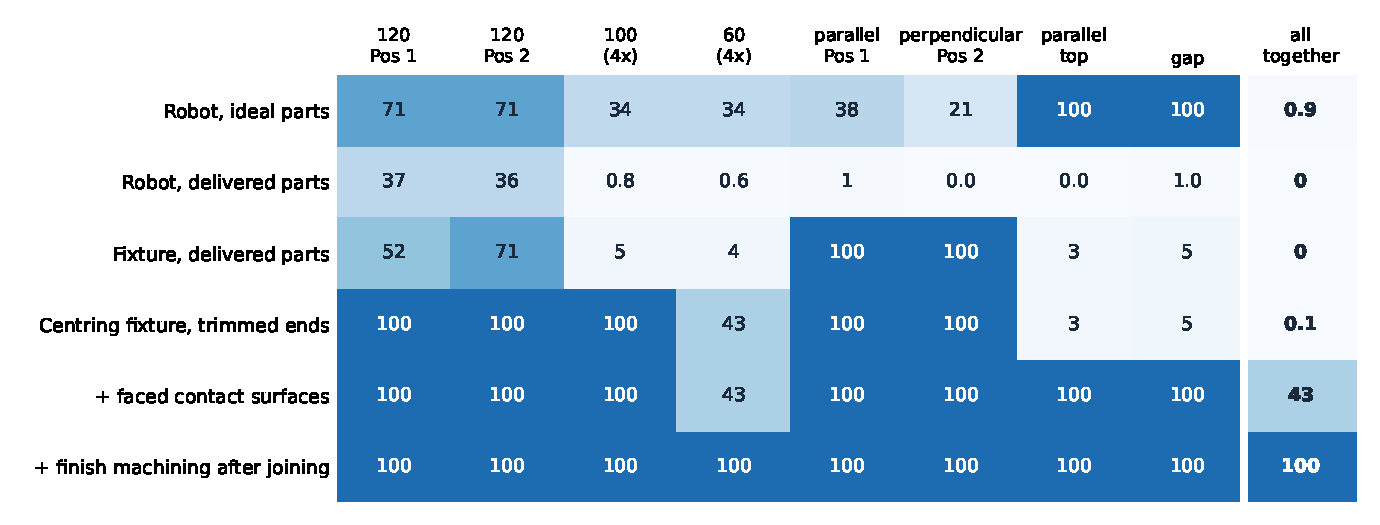
\includegraphics[width=\textwidth]{yield_matrix.pdf}
\caption{Percentage of assemblies that meet each requirement (normal distribution of part errors).}
\label{fig:yield}\end{figure}

What can be seen from Fig.~\ref{fig:yield}:
\begin{itemize}
\item Robot only: even with ideal parts the orientation and the dimensions 100 and 60 fail. This is the answer to the reality check question, the precision has to come from somewhere else.
\item With a fixture the position is good, but still almost no assembly is OK. The reason is the height of the profiles, the leg ends and the length.
\item Machining the contact surfaces solves height and gap. The dimension 60 is only OK when the ends are machined after joining, measured from the real welded frame.
\end{itemize}

The 100\% in the last row comes only from the assumed milling accuracy, welding distortion is not inside. So it means ``no geometric conflict is left'', not a real yield.

I also tried a uniform distribution instead of normal. Then the variant with machined contact surfaces goes down from 43\% to 9\%, but the last row stays at 100\%. So with machining after joining the result does not depend much on the supplier.

\section{How to reach the tolerances}
The idea is to give each accuracy level to the part of the system that can do it:

\begin{table}[H]\centering
\begin{tabular}{lll}\toprule
Level & What it does & Accuracy\\\midrule
Robots & bring the part into the capture zone & ca. 1~mm\\
Fixture & centre, straighten and hold during joining & ca. 0.01~mm\\
Machining and measuring & final reference surfaces, check & ca. 0.02~mm\\\bottomrule
\end{tabular}
\end{table}

\subsection{Fixture}
The fixture has stops on both sides of each profile which close together (centring), so the profile is located on its middle plane. With a stop only on one side, the width tolerance would move the axis. The concept is in Fig.~\ref{fig:cad}, the STEP file is in the repository.

\begin{figure}[H]\centering
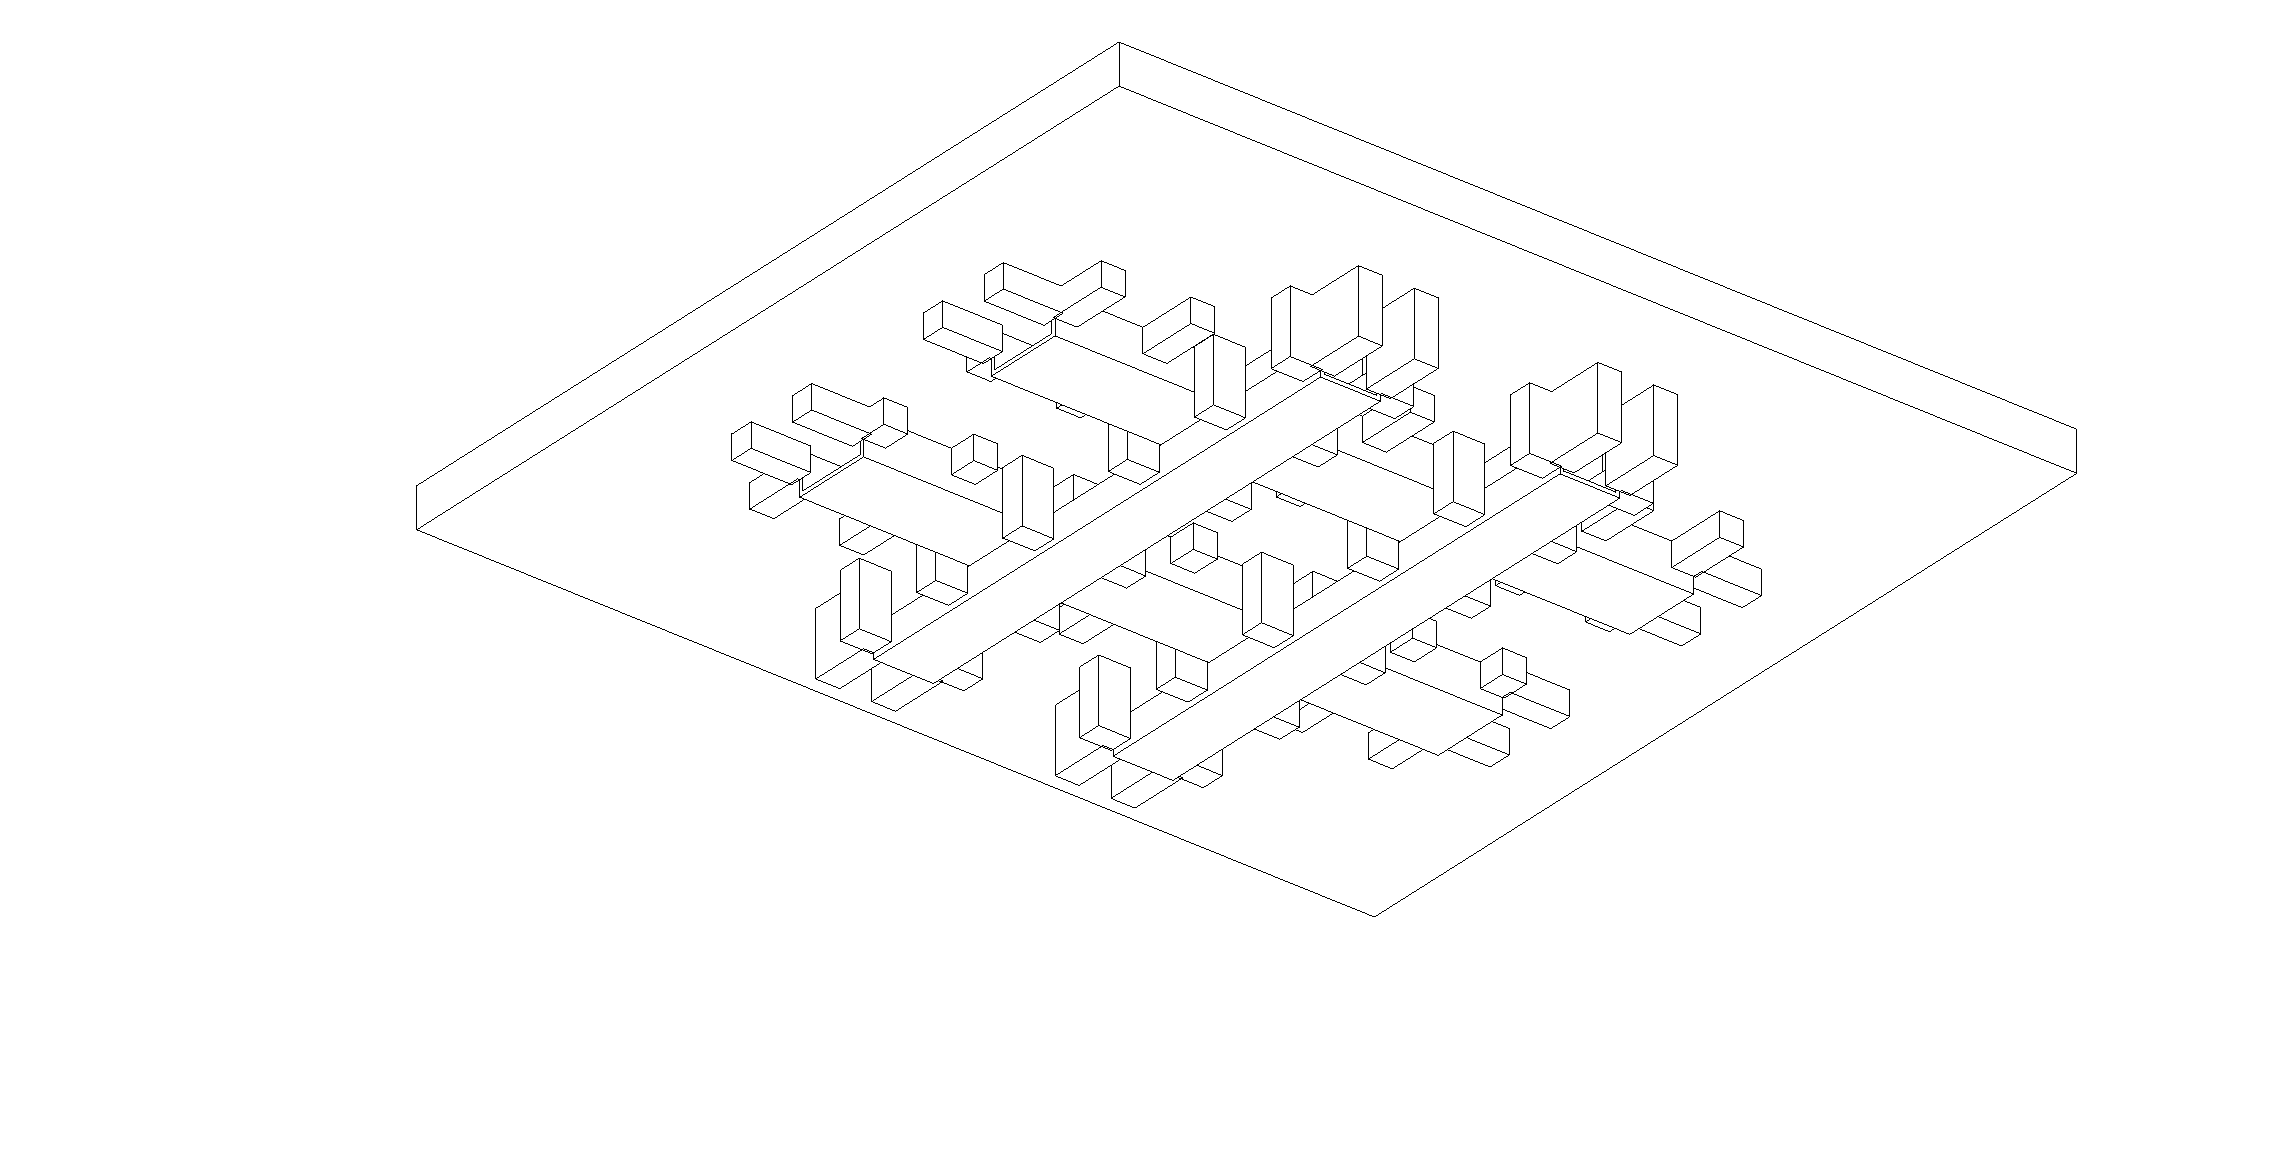
\includegraphics[width=.72\textwidth]{hash_fixture_crop.pdf}
\caption{Fixture concept. 7 stops on each Pos~1 flank, 6 on each Pos~2 flank, end stops on the legs.}
\label{fig:cad}\end{figure}

Some points for the fixture design:
\begin{itemize}
\item To straighten a bow of 0.5~mm a force of about 300~N is needed (three point bending, $F = 48EI\delta/L^3$, $I \approx 3.7\cdot10^4$~mm$^4$ for Pos~1). The xArm6 payload is 5~kg, so the robot can not do this, the clamps have to.
\item The bow left between two stops goes with $(s/L)^2$. Under Pos~2 there is Pos~1, so the stops can not be placed evenly. If they are put directly next to the Pos~1 flanks, the biggest span is 66~mm. With even spacing it would be 105~mm, and then only 48\% of the assemblies are OK in perpendicularity.
\item The stress at 300~N is only about 13~MPa, much below the yield strength. So the profile springs back after unclamping, and stays straight only as much as the welds hold it.
\item The end stops must touch the legs. A stop in the middle of the open profile goes under the web and does not touch the part.
\item Lead-in: 4~mm clearance and 7~mm chamfer on each side. The chamfer must not stick out over the stop face, otherwise it lifts the part when clamping.
\end{itemize}

\subsection{Process steps}
\begin{enumerate}
\item Incoming check of the parts: length, width, bow.
\item Machine the leg ends of Pos~2 and the top of Pos~1, leave material on the ends.
\item The robots put the parts into the fixture. First the end stops close, then the side stops, then the top clamps.
\item Welding with low and symmetric heat input. With 12~$\mu$m/(m\,K) already 13~K temperature difference gives 0.05~mm on 320~mm. That is why the fixture should be from steel and not aluminium.
\item Machining of the ends and the top of Pos~2 in one clamping, from the welded frame.
\item Measuring, and correcting the clamping and welding sequence with the results.
\end{enumerate}
If machining after welding is not allowed, another way is selective assembly: measure the width of each Pos~1 and cut each Pos~2 to the matching length.

\section{Robot cell and simulation}
The cell was simulated in MuJoCo, with the xArm6 geometry from the official UFACTORY ROS2 package. The two robots stand opposite each other, 800~mm apart, and each has its own part stacks (Fig.~\ref{fig:frames}). Each robot places one Pos~1 and then one Pos~2. Pos~2 can only be placed when both Pos~1 are in the fixture. As gripper I use a tool with two suction cups on the closed web. A magnetic gripper would also be possible, because S235 is magnetic.

At a distance of 120~mm the two wrists do not fit next to each other above the middle of the parts. So each robot grips the part 80~mm out of the middle, to its own side.

\begin{figure}[H]\centering
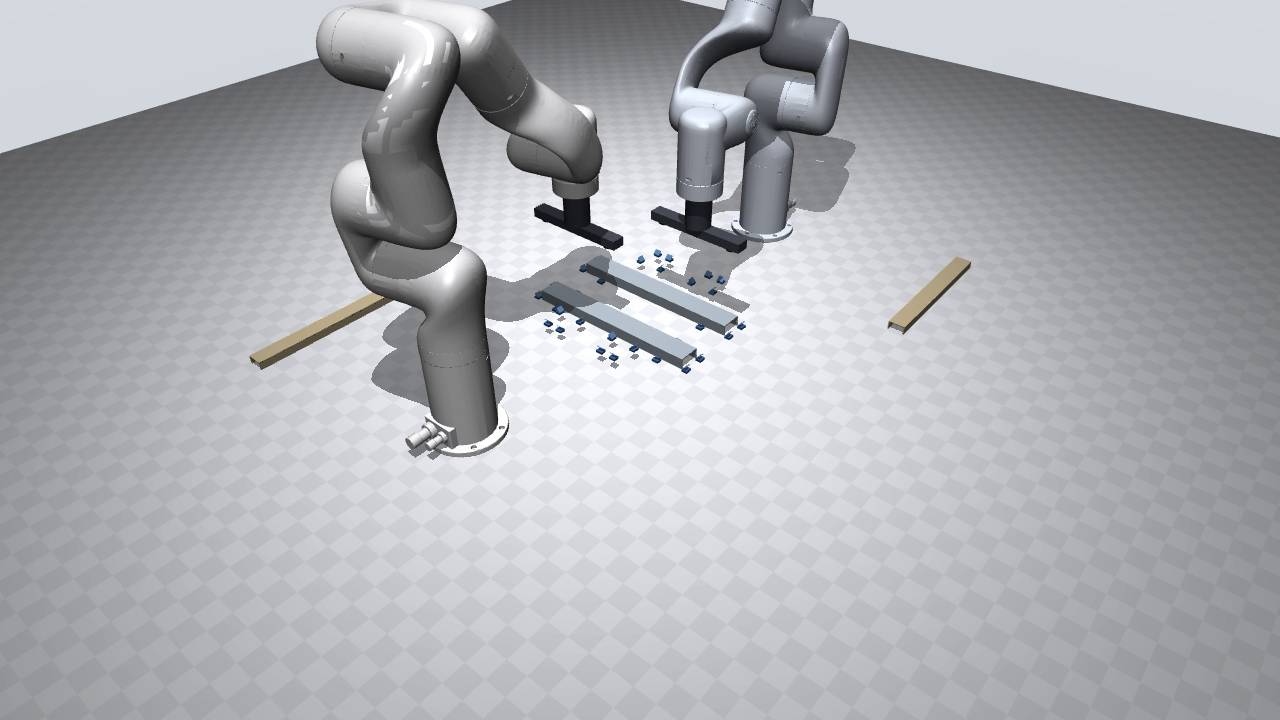
\includegraphics[width=.49\textwidth]{frame1.png}\hfill
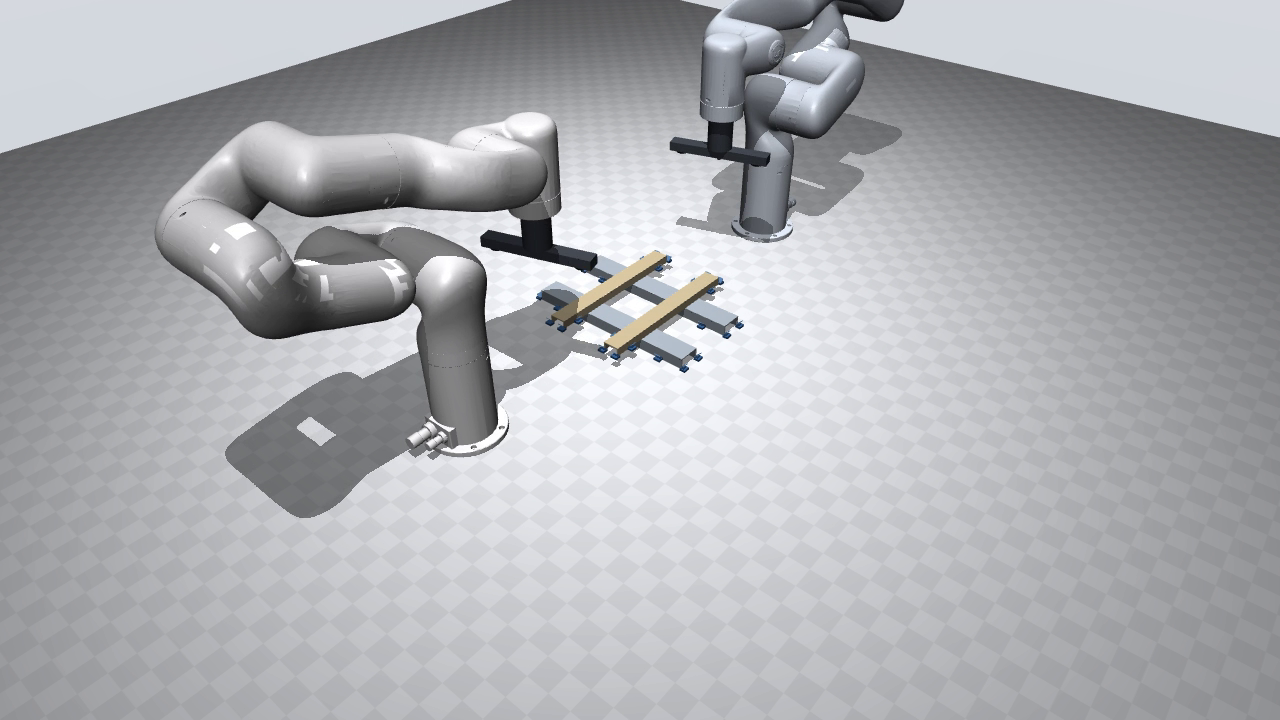
\includegraphics[width=.49\textwidth]{frame3.png}
\caption{Simulation: placing of the lower level (left) and the finished assembly (right).}
\label{fig:frames}\end{figure}

\subsection{Capture range of the fixture}
To check how much robot error the fixture can take, the parts were dropped from 12~mm above the seat with a random error up to 16~mm and $\pm1^\circ$, 600 times per part type. Then the jaws were closed. A part is counted as seated if it is within 0.1~mm and 1~mrad in the plane and 0.3~mm in height.

\begin{figure}[H]\centering
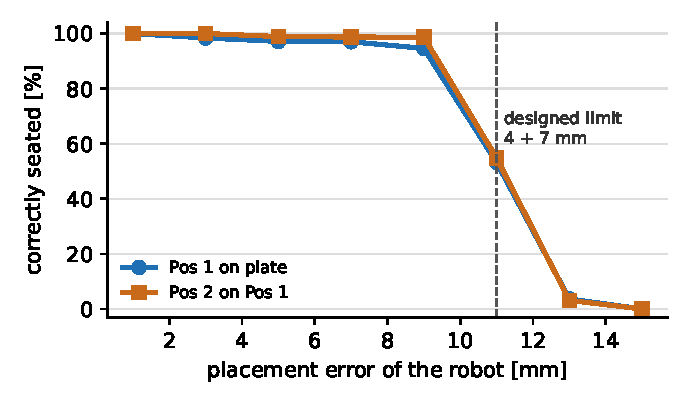
\includegraphics[width=.49\textwidth]{capture.pdf}\hfill
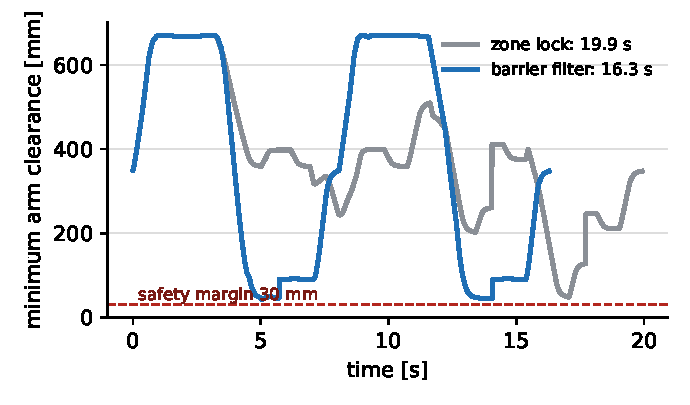
\includegraphics[width=.49\textwidth]{clearance.pdf}
\caption{Left: capture curve (60--90 tries per point). Right: smallest distance between the robots during one cycle.}
\label{fig:capture}\end{figure}

As can be seen in Fig.~\ref{fig:capture} (left), up to 10~mm error 95--100\% of the parts are seated. At 11~mm it drops, this is exactly clearance plus chamfer. The parts stay about 0.14~mm too high because of the friction in the jaws, so top clamps are necessary. The simulation uses rigid contact, so it shows the capture geometry, but it says nothing about accuracy in micrometres.

\subsection{Two robots in one workspace}
The robots can collide above the fixture. The simple solution is a zone lock: only one robot is allowed in the common zone. As a second variant both robots move freely and a control barrier function (CBF) filter is added. $h$ is the distance between capsules around the robot links minus a safety margin of 30~mm. The joint velocity is changed as little as possible:
\begin{equation*}
\dot q^\ast = \arg\min_{\dot q} \|\dot q - \dot q_\text{nom}\|^2_W \quad \text{s.t.} \quad \dot h(q,\dot q) \ge -\alpha h
\end{equation*}
From this $h(t) \ge h(0)e^{-\alpha t}$, so if the robots start in a safe state they stay safe. The QP is solved at 100~Hz with Hildreth's method.

\begin{table}[H]\centering
\begin{tabular}{lrr}\toprule
& Zone lock & CBF filter\\\midrule
Cycle time & 19.9~s & 16.3~s\\
Smallest distance between robots & 47.8~mm & 42.1~mm\\
Filter active & -- & 3\% of the steps\\\bottomrule
\end{tabular}
\end{table}

The cycle is 18\% shorter. This comes mainly from the parallel work, the filter is active only in 3\% of the steps, it is more a safety net. With gripping in the middle of the parts the filter stopped both robots at the 30~mm margin. So it avoids the collision, but it can not solve the deadlock, the task plan itself must be feasible. Also the guarantee is only valid if the robot follows the velocity command, and it is not a replacement for a certified safety function.

\section{Calibration and placing on the real robot}
\textbf{Calibration.} For the cell the transformation between the two robot bases is needed. One touch on a plane with normal $n$ in point $p$ gives one row $[n^\top, (p\times n)^\top]$ of the measurement Jacobian. If only the plate is touched, the rank is 3, the shift in the plane and the rotation around the vertical axis can not be found. With 3-2-1 touches on the plate, a long side and an end face the rank is 6. So the datum faces of the fixture are also needed for the calibration.

\textbf{Placing.} In the simulation the part is dropped above the seat. On the real robot I would put it down with admittance control, $M\ddot e + D\dot e + Ke = f$. With $V = \frac12 \dot e^\top M \dot e + \frac12 e^\top K e$ follows $\dot V = -\dot e^\top D \dot e + \dot e^\top f$, so the robot is passive in contact and stays stable with the passive fixture.

\section{Limitations and next steps}
\begin{itemize}
\item The motion in the simulation is kinematic, with position controlled joints and without payload dynamics.
\item Twist, step of the leg ends and position in the gripper are estimated. The order of the process variants stays the same also for other values.
\item Welding distortion and springback after unclamping are not in the model. This is the biggest open risk.
\item In the simulation the fixture has only two fingers per side, the tolerance model and the CAD have the full stop layout.
\end{itemize}

Next steps on hardware: measure the repeatability with a dial gauge, do the capture test with 3D printed fixture blocks, measure the bow on some real parts, and weld test frames to see the distortion.

Code, CAD and videos (also a side by side video of both variants): [repository link].
\end{document}
